% v2-acmsmall-sample.tex, dated March 6 2012
% This is a sample file for ACM small trim journals
%
% Compilation using 'acmsmall.cls' - version 1.3 (March 2012), Aptara Inc.
% (c) 2010 Association for Computing Machinery (ACM)
%
% Questions/Suggestions/Feedback should be addressed to => "acmtexsupport@aptaracorp.com".
% Users can also go through the FAQs available on the journal's submission webpage.
%
% Steps to compile: latex, bibtex, latex latex
%
% For tracking purposes => this is v1.3 - March 2012

\documentclass[prodmode,acmtecs]{acmsmall} % Aptara syntax

\usepackage{graphicx}
\usepackage{caption}
\usepackage{subfigure}
\usepackage{setspace}
\usepackage{tabulary}
\usepackage{fancybox}

% font in listings
\usepackage{courier}

\makeatletter
\newenvironment{CenteredBox}{% 
\begin{Sbox}}{% Save the content in a box
\end{Sbox}\centerline{\parbox{\wd\@Sbox}{\TheSbox}}}% And output it centered
\makeatother

\let\proof\relax
\let\endproof\relax
\usepackage{amsthm}
\newcommand{\specialcell}[2][c]{%
  \begin{tabular}[#1]{@{}c@{}}#2\end{tabular}}

\usepackage{lineno}
\usepackage{xfrac}

% Theorems, definitions, lemmas, etc
\newtheorem{Def}{Definition}
\newtheorem{Prop}{Proposition}

\usepackage{alltt}
\renewcommand{\ttdefault}{txtt}

\usepackage{listings}
\lstset{language=C, breaklines=true, mathescape}

\usepackage[cmex10]{amsmath}
\usepackage{url}



% Metadata Information
%\acmVolume{9}
%\acmNumber{4}
%\acmArticle{39}
%\acmYear{2010}
%\acmMonth{3}

% Document starts
\begin{document}

% Page heads
\markboth{F. Luporini et al.}{Optimal Finite Element Integration}

% Title portion
\title{Optimal Finite Element Integration}
\author{Fabio Luporini
\affil{Imperial College London}
David A. Ham
\affil{Imperial College London}
Paul H.J. Kelly
\affil{Imperial College London}}

\begin{abstract}
...
\end{abstract}

\category{G.1.8}{Numerical Analysis}{Partial Differential Equations -
  Finite element methods}

\category{G.4}{Mathematical Software}{Parallel and vector implementations}

\terms{Design, Performance}

\keywords{Finite element integration, local assembly, compilers, optimizations, SIMD vectorization}

\acmformat{Fabio Luporini, David A. Ham, and Paul   H. J. Kelly, 2015. Optimal Finite Element Integration.}

% At a minimum you need to supply the author names, year and a title.
% IMPORTANT: Full first names whenever they are known, surname last,
% followed by a period.  In the case of two authors, 'and' is placed
% between them.  In the case of three or more authors, the serial
% comma is used, that is, all author names except the last one but
% including the penultimate author's name are followed by a comma, and
% then 'and' is placed before the final author's name.  If only first
% and middle initials are known, then each initial is followed by a
% period and they are separated by a space.  The remaining information
% (journal title, volume, article number, date, etc.) is
% 'auto-generated'.

\begin{bottomstuff}

This research is partly funded by the MAPDES project, by the
Department of Computing at Imperial College London, by EPSRC through
grants EP/I00677X/1, EP/I006761/1, and EP/L000407/1, by NERC grants
NE/K008951/1 and NE/K006789/1, by the U.S.  National Science
Foundation through grants 0811457 and 0926687, by the U.S. Army
through contract W911NF-10-1-000, and by a HiPEAC collaboration
grant. The authors would like to thank Dr. Carlo Bertolli,
Dr. Lawrence Mitchell, and Dr. Francis Russell for their invaluable
suggestions and their contribution to the Firedrake project.

Author's addresses: Fabio Luporini $\&$ Paul H. J. Kelly, Department of Computing,
Imperial College London; David A. Ham, Department of Computing and
Department of Mathematics, Imperial College London; 
\end{bottomstuff}

\maketitle


\section{Introduction}

The need for rapidly implementing high performance, robust, and portable finite element methods has led to approaches based on automated code generation. This has been proved successful in the context of the FEniCS (\cite{Fenics}) and Firedrake (\cite{firedrake-code}) projects, which have become increasingly popular over the last years. In these frameworks, the weak variational form of a problem is expressed at high-level by means of a domain-specific language. The mathematical specification is manipulated by a form compiler, which then generates a representation of assembly operators. By applying these operators to an element in the discretized domain a local matrix and a local vector, which represent the contributions of that element to the equation solution, are computed. The code for assembly operators should be high performance: as the complexity of a variational form increases, in terms of number of derivatives, pre-multiplying functions, or polynomial order of the chosen function spaces, the operation count increases, thus making assembly covering a significant fraction of the overall runtime. 

As demonstrated across a great deal of works, automating the generation of such high performance implementations poses several challenges. This is a result of the complexity inherent to the mathematical expressions involved in the numerical integration, which varies from problem to problem, and the particular structure of the loop nests enclosing the integrals. General-purpose compilers, such as \emph{GNU's} and \emph{Intel's}, fail at exploiting the structure inherent the expressions, thus producing sub-optimal code (i.e., code which performs more floating-point operations, or "flops", than necessary). Research compilers, for instance those based on polyhedral analysis of loop nests such as PLUTO (\cite{PLUTO}), focus on aggressive loop optimizations for cache locality, so they are not particularly helpful in our context. The lack of suitable third-party tools has led to the development of a number of domain-specific transformation systems or synthesizers. In~\citeN{quadrature1}, it is shown how automated code generation can be leveraged to introduce domain-specific optimizations that a user should not be expected to write ``by hand''. In~\citeN{Kirby-FEM-opt} and~\citeN{Francis}, mathematical reformulations of finite element integration are studied with the aim of minimizing the operation count. In~\citeN{Luporini}, the effects and the interplay of generalized code motion and a set of low-level optimizations are analysed. There is also an on-going effort to produce a novel form compiler, and therefore a novel code generation system for assembly operators, called UFLACS (\cite{Uflacs}). 

In spite of a considerable research effort, still there is no answer to one fundamental question: can we automatically generate an implementation of a form which is optimal in the number of flops executed? With this paper, we aim to make a first step in the direction of solving this problem.

We summarize the contributions of this research as follows
\begin{itemize}
\item We characterize flop-optimality in a loop nest and we instantiate this concept to finite element integration. As part of this construction, we establish the notion of sharing and demonstrate that sharing can always be eradicated from the loop nests we are interested in.
\item We provide an incremental, constructive proof that optimal implementations can be synthesized by analyzing each monomial appearing in a form
\item We implemented the theory in our compiler, COFFEE\footnote{...}, which is the default optimization system in the Firedrake framework. Our implementation is general: we can apply our results to any forms expressible in Firedrake (and, theoretically, in FEniCS too).
\item We provide an unprecedented (for extension) performance evaluation comparing several code transformation/synthesizers systems in a wide range of forms of increasing complexity, which is essential to demonstrate our optimality claim.
\item We comment on the cases in which our characterization of optimality becomes weaker, and intuitions about how we deal with (i.e., optimize) them
\item We enrich the set of low-level transformations described in~\citeN{Luporini}
\end{itemize}


\section{Preliminaries}
\label{sec:background}

%is the computation of contributions of a specific cell in the discretized domain to the linear system which yields the PDE solution. The process consists of numerically evaluating problem-specific integrals to produce a matrix and a vector [Olgaard and Wells 2010; AMCG 2010], whose sizes depend on the order of the method. This operation is applied to all cells in the discretized domain. In this work we focus on local matrices, or “element matrices”, which are more costly to compute than element vectors.

We review finite element integration and possible implementations using notation and examples adopted in~\cite{quadrature1} and~\cite{Francis}. 

We consider the weak formulation of a linear variational problem
\begin{equation}
\begin{split}
Find\ u\ \in U\ such\ that \\
a(u, v) = L(v), \forall v \in V
\end{split}
\end{equation}
where $a$ and $L$ are, respectively, a bilinear and a linear form. The set of \textit{trial} functions $U$ and the set of \textit{test} functions $V$ are discrete function spaces. For simplicity, we assume $U = V$ and $\lbrace \phi_i \rbrace$ be the set of basis functions spanning $U$. The unknown solution $u$ can be approximated as a linear combination of the basis functions $\lbrace \phi_i \rbrace$. From the solution of the following linear system it is possible to determine a set of coefficients to express $u$
\begin{equation}
A\textbf{u} = b
\end{equation}
in which $A$ and $b$ discretize $a$ and $L$ respectively:
\begin{equation}
\centering
\begin{split}
A_{ij} = a(\phi_i(x), \phi_j(x)) \\
b_i = L(\phi_i(x))
\end{split}
\end{equation}
The matrix $A$ and the vector $b$ are computed in the so called assembly phase. Then, in a subsequent phase, the linear system is solved, usually by means of an iterative method, and $\textbf{u}$ is eventually evaluated. 

We focus on the assembly phase, which is often characterized as a two-step procedure: \textit{local} and \textit{global} assembly. Local assembly is the subject of the paper: this is about computing the contributions that an element in the discretized domain provide to the approximated solution of the equation. Global assembly, on the other hand, is the process of suitably ``inserting'' such contributions in $A$ and $b$. 

Without loss of generality, we illustrate local assembly in a concrete example; that is, the evaluation of the local element matrix for a Laplacian operator. Consider the weighted Laplace equation
\begin{equation}
- \nabla \cdot (w \nabla u) = 0
\end{equation}
in which $u$ is unknown, while $w$ is prescribed. The bilinear form associated with the weak variational form of the equation is:
\begin{equation}
a(v, u) = \int_\Omega w \nabla v \cdot \nabla u\ \mathrm{d}x
\end{equation}
The domain $\Omega$ of the equation is partitioned into a set of cells (elements) $T$ such that $\bigcup T = \Omega$ and $\bigcap T = \emptyset$. By defining $\lbrace \phi_i^K \rbrace$ as the set of local basis functions spanning $U$ on the element $K$, we can express the local element matrix as
\begin{equation}
\label{stiffness}
A_{ij}^K = \int_K w \nabla \phi_i^K \cdot \nabla \phi_j^K\ \mathrm{d}x
\end{equation}
The local element vector $L$ can be determined in an analogous way. 
%From the computational perspective, its evaluation is however less expensive than that of $A$.

\subsection{Quadrature Mode}
Quadrature schemes are conveniently used to numerically evaluate $A_{ij}^K$. For convenience, a reference element $K_0$ and an affine mapping $F_K : K_0 \rightarrow K$ to any element $K \in T$ are introduced. This implies a change of variables from reference coordinates $X_0$ to real coordinates $x = F_K (X_0)$ is necessary any time a new element is evaluated. The numerical integration routine based on quadrature representation over an element $K$ can be expressed as follows
\begin{equation}
\label{eq:quadrature}
\scriptsize
A_{ij}^K = \sum_{q=1}^N \sum_{\alpha_3=1}^n \phi_{\alpha_3}(X^q)w_{\alpha_3} \sum_{\alpha_1=1}^d \sum_{\alpha_2=1}^d \sum_{\beta=1}^d \frac{\partial X_{\alpha_1}}{\partial x_{\beta}} \frac{\partial \phi_i^K(X^q)}{\partial X_{\alpha_1}} \frac{\partial X_{\alpha_2}}{\partial x_{\beta}} \frac{\partial \phi_j^K(X^q)}{\partial X_{\alpha_2}} det F_K' W^q
\end{equation}
where $N$ is the number of integration points, $W^q$ the quadrature weight at the integration point $X^q$, $d$ is the dimension of $\Omega$, $n$ the number of degrees of freedom associated to the local basis functions, and $det$ the determinant of the Jacobian matrix used for the aforementioned change of coordinates.  

% Magari la summation sui coefficients la sputo dentro? che dici?

\subsection{Tensor Contraction Mode}
Starting from Equation~\ref{eq:quadrature}, exploiting basic mathematical properties we can rewrite the expression as
\begin{equation}
\label{eq:tensor}
\scriptsize
A_{ij}^K = \sum_{\alpha_1=1}^d \sum_{\alpha_2=1}^d \sum_{\alpha_3=1}^n det F_K' w_{\alpha_3} \sum_{\beta=1}^d \frac{X_{\alpha_1}}{\partial x_{\beta}} \frac{\partial X_{\alpha_2}}{\partial x_{\beta}} \int_{K_0} \phi_{\alpha_3} \frac{\partial \phi_{i_1}}{\partial X_{\alpha_1}} \frac{\partial \phi_{i_2}}{\partial X_{\alpha_2}} dX.
\end{equation}
A generalization of this transformation has been proposed in~\cite{Kirby:TC}. By only involving reference element terms, the integral in the equation can be pre-evaluated and stored in a temporary. The evaluation of the local tensor can then be abstracted as
\begin{equation}
A_{ij}^K = \sum_{\alpha} A_{i_1 i_2 \alpha}^0 G_{K}^\alpha
\end{equation}
in which the pre-evaluated "reference tensor" $A_{i_1 i_2 \alpha}$ and the cell-dependent "geometry tensor" $G_{K}^\alpha$ are exposed. 

\subsection{Qualitative Comparison}
Depending on the form being considered, the relative performance of the two modes, in terms of number of operations executed, can vary even quite dramatically. The presence of derivatives or coefficient functions in the input form tends to increase the size of the geometry tensor, making the traditional quadrature mode increasingly more indicate for "complex" forms. On the other hand, speed ups from adopting tensor mode can be significant in a wide class of forms in which the geometry tensor remains "sufficiently small". 

These two modes have been implemented in the FEniCS Form Compiler. In this compiler, a simple heuristic is used to choose the most suitable mode for a given form. It consists of analysing each monomial in the form, counting the number of derivatives and coefficient functions, and checking if this number is greater than a constant found empirically~\cite{Fenics}. We will later comment on the efficacy of this approach (Section~\ref{sec:optimal-synthesis}. For the moment, we just recall that one of the goals of this research is to produce an intelligent system that is capable of selecting the optimal mode at the monomials level -- no heuristics, no "global" choice of the mode for all monomials in the form -- without affecting the cost of code generation.

\section{Optimality of Loop Nests}
\label{sec:optimal-impl}

In this section, we provide a characterization of optimality for loop nests of various nature. In order to make the document self-contained, we start with reviewing basic compiler terminology.

\begin{Def}[Perfect and imperfect loop nests]
A loop nest is said to be \textit{perfect} when non-loop statements appear only in the body of the innermost loop. If this condition does not hold, a loop nest is said \textit{imperfect}. 
\end{Def}

A straightforward property of perfect nests is that hoisting invariant expressions from the innermost loop to the preheader (i.e., the block that precedes the entry point of the nest) is a safe transformation. We will make use of this property.

% In the following, we should represent loops by their iteration variable.

\begin{Def}[Linear loop]
A loop $L$ defining the iteration space $I$ through the iteration variable $i$, or simply $L_i$, is \textit{linear} if all expressions appearing in the body of $L$ that use $i$ to access some memory locations are linear functions over $I$.
\end{Def}

In this work, we are particularly interested in the following class since it naturally arises from the math described in Section~\ref{sec:background}.

\begin{Def}[Perfect multilinear loop nest]
A \textit{perfect multilinear} loop nest of arity $n$ is a perfect nest composed of $n$ loops, in which all of the expressions appearing in the body of the innermost loop are linear in each loop $L_i$ separately.
\end{Def}

Note that perfect multilinear loop nests could actually be rooted in deeper, possibly imperfect loop nests. In fact, we will focus on this particular structure. 

We introduce the fundamental notion of sharing.

\begin{Def}[Sharing]
A loop $L_i$ presents \textit{sharing} if it contains at least two expressions depending on $i$ that are symbolically identical. 
\end{Def}

Figure~\ref{code:multi_loopnest} shows an example of a trivial multilinear loop nest of arity $n=2$ with sharing along dimension $k$.

\begin{figure}[h]\begin{CenteredBox}
\lstinputlisting[basicstyle=\footnotesize\ttfamily]{listings/multilinear_loopnest.code}
\end{CenteredBox}\caption{Multilinear loop nest with sharing}\label{code:multi_loopnest}\end{figure}

We now have the ingredients to formulate a simple yet fundamental result.

\begin{Prop}
\label{prop:share-removal}
Sharing in a perfect multilinear loop nest $LN = [L_{i_{0}}, L_{i_{1}}, ..., L_{i_{n-1}}]$ can always be eliminated.
\end{Prop}
\begin{proof}
The demonstration is by construction and exploits linearity. We want to transform $LN$ into $LN'$ such that there is no sharing is any $L_i \in LN'$. Starting from the innermost loop $L_{i_{n-1}}$, the expressions are ''flattened'' by expanding all products involving terms depending on $L{i_{n-1}}$. Being on the same level of the expression tree, such terms can then be factorized. Due to linearity, each factored product only has one term depending on $L_{i_{n-1}}$, and such term is now unique in the expression. The other terms, independent of $L_{i_{n-1}}$, are, by definition, loop-invariant, and as such can be hoisted at the level of $L_{i_{n-2}}$. This procedure can be applied recursively up to $L_{i_{0}}$: multilinearity allows factorization at each level; perfectness ensures hoisting is always safe.
\end{proof}

This result will be essential to prove that optimality, characterized as follows, can structurally be reached in this class of loops.

\begin{Def}[Optimality of a multilinear loop nest]
The synthesis of a multilinear loop nest is \textit{optimal} if the amount of operations performed in the innermost loop is minimum.
\end{Def}

In other words, optimality implies there is no other synthesis able to further decrease the number of operations in the innermost loop. Note that this definition does not take into account memory requirements. If the loop nest were memory-bound -- the ratio of operations to bytes transferred from memory to the CPU being too low -- then speaking of ''optimality'' would clearly make no sense. In the following, we assume to operate in a CPU-bound regime, in which arithmetic-intensive expressions need be evaluated. This suits the context of finite element integration.

A second result follows.
\begin{Prop}
\label{prop:optimal-mln}
A perfect multilinear loop nest $LN$ can always be reduced to optimal form.
\end{Prop}
\begin{proof}
By construction. Loop-dependent terms are logically grouped into $n$ disjoint sets $S_i$, each $S_i$ containing all terms depending on $L_i$. These sets are sorted in descending order based on their cardinality. By establishing a one-to-one mapping between set indices and loop indices, we produce a new loop permutation. The loop permutation is semantically correct because of perfectness. In this new order, loops are placed such that as going down the nest, $L_i$ is characterized by less unique terms than $L_{i-1}$. Starting from $L_{i_{n-1}}$, we can apply the sharing-removal procedure described in Proposition~\ref{prop:share-removal}. This renders $L_{i_{n-1}}$ optimal. In particular, the number of operations is equal to $LN_{ops} = \# S_{i_{n-1}} + (\# S_{i_{n-1}} - 1)$, in which the second term represents the cost of summing the $\# S_{i_{n-1}}$ terms.
\end{proof}

For example, by applying the construction described in Proposition~\ref{prop:optimal-mln} to the code in Figure~\ref{code:multi_loopnest}, we obtain the optimal form in Figure~\ref{code:multi_loopnest_optimal}.

\begin{figure}[h]\begin{CenteredBox}
\lstinputlisting[basicstyle=\footnotesize\ttfamily]{listings/multilinear_loopnest_opt.code}
\end{CenteredBox}\caption{Multilinear loop nest in optimal form}\label{code:multi_loopnest_optimal}\end{figure}

We now consider a wider class of loop nests in which perfectness and multilinearity apply to a sub-nest only. Consider the example in Figure~\ref{code:loopnest}. 

\begin{figure}[h]\begin{CenteredBox}
\lstinputlisting[basicstyle=\footnotesize\ttfamily]{listings/loopnest.code}
\end{CenteredBox}\caption{Loop nest example}\label{code:loopnest}\end{figure}

The imperfect nest $LN=[L_e, L_i, L_j, L_k]$ comprises a reduction loop $L_i$ and a perfect doubly nested loop $[L_j, L_k]$, which we assume to be multilinear. The right hand side of the statement computing the multidimensional array \texttt{A} is a generic expression \texttt{F} including standard arithmetic operations such as addition and multiplication. We observe that \texttt{F} might contain sub-expressions that depend on a subset of loops only and, as such, hoistable outside of $LN$ as long as data dependencies are preserved (note that $LN$ is imperfect). One could think of searching for sub-expressions independent of $L_e$, for which the reduction could be pre-evaluated, thus obtaining a decrease proportional to $M$ in the operation count. However, finding or exposing such reducible sub-expressions requires, in general, a full exploration of the expression tree transformation space. This is obviously challenging, and so is the problem of synthesizing an optimal $LN'$ starting from $LN$. Even though we assumed we could generate $LN'$ in non-exponential time, the following issues should be addressed
\begin{itemize}
\item as opposed to what happens with hoisting in perfect multilinear loop nests, the temporary variable size would be proportional to the number of non-reduction loops crossed (in the example, $N \cdot O$ for sub-expressions depending on $[L_i, L_j, L_k]$ and $L \cdot N \cdot O$ for those depending on $[L_e, L_i, L_j, L_k] $). This might shift the loop nest from a CPU-bound to a memory-bound regime, which might be counter-productive for actual runtime;
\item the transformations exposing multi-invariant sub-expressions could require expansion and factorization. In terms of number of operations, the save originating from the elimination of the reduction loop could be overwhelmed by the increase in arithmetic complexity of $L_k$ (e.g., expansion can increase the operation count, e.g. $A(B+C) = AB + AC$).
\end{itemize}

We then refine our definition of optimality for generic loop nests as follows

\begin{Def}[Optimality of a loop nest]
\label{def:optimality}
The synthesis of a loop nest is \textit{optimal} if, under a set of memory constraints \texttt{C}, the total amount of operations performed in all innermost loops is minimum.
\end{Def}

Note how the definition contemplates the possibility for a nest to have multiple innermost loops. In fact, multiple sub-nests could be rooted in the outermost loop, either because part of the input or result of suitable transformations.

\section{Synthesis of Optimal Loop Nests in Finite Element Integration}
\label{sec:optimal-synthesis}

In this section, we instantiate Definition~\ref{def:optimality} in our domain of interest, finite element integration. This will require reasoning at two different levels of abstraction: the math, in terms of the multilinear forms arising from the weak variational formulation of a problem, which we reviewed in Section~\ref{sec:background}; and the (partly multilinear) loop nests implementing such forms.

Our point of departure is the example loop nest in Figure~\ref{code:loopnest}. This loop nest is actually a simplified view of a typical bilinear form implementation. $L_e$ represents iteration over the elements of a mesh; $L_i$ derives from using numerical quadrature; $[L_j, L_k]$ implement the computation over test and trial functions. We deliberately omitted useless portions of code to not hinder readability (e.g. matrix insertion) and to avoid tying our discussion to specific forms (e.g. \texttt{F} is unspecified).

From domain knowledge, we make the following observations. 1) $L >>> M, N, O$; that is, the number of elements $L$ is typically order of magnitude larger than both quadrature points ($M$) and degrees of freedom ($N$ and $O$ for test and trial functions); 2) $[L_j, L_k]$ (or simply $L_j$ with a linear form) is perfect and multilinear; this naturally descends from the translation of Equation~\ref{eq:quadrature} into a loop nest. 

% maybe say somewhere the order of the loop nest eijk is just the most natural --- the other present worse data locality for example

\subsection{Memory constraints}
\label{sec:mem-const}
The fact that the iteration space of $L_e$ is so larger than that of other loops suggests we should be cautious when hoisting out of $LN$. Imagine a time stepping loop $L_t$ wraps $LN$. One could then think of identifying time-invariant sub-expressions that access both geometry and reference element terms and pre-evaluate them within $L_t$. Unless adopting complex engineering solutions (e.g. aggressive blocking), which are practically difficult to devise and maintain, this kind of code motion increases the working set by $O(L)$. It is our opinion, therefore, that the drop in number of operations would be overwhelmed, from the run-time viewpoint, by the larger memory pressure.

A second, more general observation is that, for certain forms and discretizations, aggressive hoisting can make the working set exceed the size of "some level of local memory" (e.g. the last level of private cache on a conventional CPU, the shared memory on a GPU). We will provide precise details about this in the following sections. For the moment, and just as one of many possible examples, note that applying tensor contraction mode (see Section~\ref{sec:background}), which essentially means lifting code outside of $L_e$, requires a set of temporary arrays of size $N\cdot O$; with some discretizations, this can break the local memory threshold.  

Based upon these considerations, we add two constraints to $C$ (see Definition~\ref{def:optimality})  
\begin{enumerate}
\item The size of a temporary due to code motion cannot be bigger than the size of the multilinear loop nest iteration space. 
\item The total size of the hoisted temporaries cannot exceed a threshold \texttt{$T_H$}
\end{enumerate}
A corollary of $C1$ is that hoisting expressions involving geometry terms outside of $L_e$ becomes forbidden.

\subsection{Minimizing the Operation Cost}
Definition~\ref{def:optimality} states that a necessary condition for a loop nest synthesis to be optimal is that the number of operations in all innermost loops is minimum. We now discuss how we can systematically achieve this.

Eliminating sharing from the inner multilinear loops does not suffice. In fact, as suggested in Section~\ref{def:optimality}, we wonder whether, and under what transformations, the reduction imposed by $L_i$ could be pre-evaluated, thus reducing the operation count.

To answer this question, we make use of a result -- the foundation of tensor contraction mode -- from~\citeN{Kirby:TC}. Essentially, multilinear forms can be seen as sums of monomials, each monomial being an integral over the equation domain of products (of derivatives) of functions from discrete spaces; such monomials can always be reduced to a product of two tensors (see Section~\ref{sec:background}). We interpret this result at the loop nest level: with the input as in Figure~\ref{code:loopnest}, we can always dissect \texttt{F} into distinct sub-expressions (the monomials). Each sub-expression is then factorized so as to split constant from $[L_i, L_j, L_k]$-dependent terms, the latter ones are hoisted outside of $LN$, and finally pre-evaluated into temporaries. As part of this pre-evaluation, the reduction induced by $L_i$ vanishes. In the following, we simply refer to this special sort of code hoisting as "\textit{pre-evaluation}". 

The challenge is to understand when, and for which monomials, pre-evaluation is profitable. We propose an algorithm and a discussion of its optimality.

The intuition of the algorithm for optimal loop nest synthesis is shown in Figure~\ref{code:intuition}. 

% local optimization of monomials
% local sharing elimination
% global sharing elimination

\begin{figure}[h]
\begin{lstlisting}[basicstyle=\small\ttfamily, frame=single]
dissect the input expression into monomials
for each monomial M:
  $\theta_{w}$ = estimate operation count with pre-evaluation
  $\theta_{wo}$ = estimate operation count without pre-evaluation
  if $\theta_{w}$ < $\theta_{wo}$ and memory constraints satisfied:
    mark M as candidate for pre-evaluation
for each monomial M:
  if M does not share terms with M$'$, an unmarked monomial:
    extract M into a separate loop nest
    apply pre-evaluation to M
for each expression:
  remove sharing    
\end{lstlisting}
\caption{Intuition of the main algorithm}
\label{code:intuition}
\end{figure}

The point of departure consists of understanding the impact, as number of operations saved or introduced, of pre-evaluation. This is studied "locally"; that is, for each monomial, in isolation. If we estimate that, for a given monomial, pre-evaluation will decrease the operation count, then the corresponding sub-expression is extracted, a sequence of transformation steps -- involving expansion, factorization, code motion -- takes place (details in Section~\ref{sec:codegen}), and the evaluation eventually performed. The result is a set of $n$-dimensional tables (these can be seen as "slices" of the reference tensor at the math level), $n$ being the arity of the multilinear form. Identical tables are mapped to the same temporary. Eventually, sharing is removed from the resulting expressions by applying a procedure as described in Proposition~\ref{prop:optimal-mln}. The transformed loop nest is as in Figure~\ref{code:loopnest-opt}. 

\begin{figure}[h]\begin{CenteredBox}
\lstinputlisting[basicstyle=\footnotesize\ttfamily]{listings/loopnest_opt.code}
\end{CenteredBox}\caption{Optimized Loop nest example}\label{code:loopnest-opt}\end{figure}

Before elaborating on the profitability of pre-evaluation, we need to discuss under which conditions this approach, based on a "local analysis" of monomials, is optimal. 

\begin{Prop}
\label{prop:optimal-approach}
Consider an expression comprising a set of monomials $M$. Let $P$ be the set of pre-evaluated monomials, determined as described in Figure~\ref{code:intuition}, and be $Z = M \setminus P$. Assume that:
\begin{enumerate}
\item the cost function employed is optimal; that is, it predicts correctly whether pre-evaluation is profitable or not for a monomial
\item pre-evaluating distinct monomials does not produce identical tables
\item monomials in $P$ do not share terms
\end{enumerate} 
Then, the loop nest $LN$ is optimal under memory constraints $C$, once sharing is removed.
\end{Prop}
\begin{proof}
We first comment on the assumptions. 1) How to create an optimal cost function is discussed in Section~\ref{sec:op_count}. 2) A pathological case due to symmetries in basis functions, which in practice rarely happens. 3) This could occur in complex forms with several monomials; for simplicity, we ignore this situation (otherwise, a "global" analysis of the monomials would be required).

We distinguish two classes of loop nests rooted in $LN$: $[L_e, L_j, L_k]$, for the pre-evaluated monomials in $P$, and $[L_e, L_i, L_j, L_k]$, enclosing the remaining monomials in $Z$. Since they only differ for the presence of $L_i$, we relieve notation by omitting all shared loops when discussing operation counts. In particular, we use $I$ to refer to the iteration space size of $L_i$. The operation count of what we are proving to be the optimal $LN$ synthesis is, therefore, $LN_{ops} = LN_{ops_1} + LN_{ops_2} = \sum_{\alpha}^{\# P} p_{\alpha} + I \sum_{\beta}^{\# Z} z_{\beta}$, where $p_{\alpha}$ and $z_{\beta}$ represent the operation cost of monomials in $P$ and $Z$, respectively.

We start noting that, as explained in Section~\ref{sec:mem-const}, $C$ imposes constraints on hoisting. This narrows the proof to demonstrating the following: A) pre-evaluating any $Z_P: Z_P \subseteq Z$ would increase $LN_{ops}$; B) not pre-evaluating any $P_Z: P_Z \subseteq P$ would increase $LN_{ops}$.

A) We prove that $LN_{ops}' = LN_{ops_1}' + LN_{ops_2}' > LN_{ops}$. It is rather obvious that $LN_{ops_1}' \geq LN_{ops_1}$ (it is equal only if, trivially, $Z_P = \emptyset$). We note that if monomials in $Z_P$ share symbols with $\overline{Z} = Z \setminus Z_P$, then we have $LN_{ops_2}' = LN_{ops_2}$, so our statement is true. If, on the other hand, at least one monomial does not share any symbols, we obtain $LN_{ops_2}' < LN_{ops_2}$ or, equivalently, $LN_{ops_2}' = LN_{ops_2} - I \cdot\delta$. What we have to show now is that even by exposing more pre-evaluations, $LN_{ops_1}' \geq LN_{ops_1} +  I \cdot\delta$ holds. This is indeed the case since we rely on assumption 2, which ensures the uniqueness of the pre-evaluated tables (i.e., the absence of sharing) and, therefore, the optimality of $LN$. 

B) In absence of sharing, the statement is trivially true since we would have $LN_{ops_2}' > LN_{ops_2}$, with the cost function being optimal by assumption. Assumption 3 guarantees there can be no sharing within $P_Z$, which avoids subtle cases wherein pre-evaluation would result sub-optimal due to destroying sharing-removal opportunities. The last case we have to consider is when $p \in P_Z$ shares at least one term with $z \in Z$. This situation cannot actually occur by construction: all candidates for pre-evaluation sharing terms with monomials in $Z$ are "declassed" from $P$ to $Z$: the rationale is that we would have to pay anyway the presence of the shared terms in the innermost loop due to $z$, so aggregating $p$ in $Z$ does not increase the operation count. 
\end{proof}

\subsection{A-Priori Operation Counting}
\label{sec:op_count}
It remains to tie one loose hand: the construction of the pre-evaluation cost function. We introduce the cost function $\theta : M \to \mathbb{N} \times \mathbb{N}$ that, given a monomial, returns two natural numbers representing the optimal operation count without ($\theta_{wo}$) and with ($\theta_{w}$) pre-evaluation. Since $\theta$ is expected to be used by a compiler to drive the transformation process, requirements are simplicity and velocity.  

We can easily predict $\theta_{wo}$ thanks to our key property, linearity. As explained in Proposition~\ref{prop:optimal-mln}, a simple analysis suffices to obtain the cost of a  sharing-free multilinear loop nest, namely $MLN_{ops}$. Then, assuming $I$ to be the size of the $L_i$ iteration space, we simply have that $\theta_{wo} = MLN_{ops} \cdot I$.

For $\theta_{w}$, things are more complicated. We first need to account for the presence of (derivatives of) coefficients to estimate the \textit{increase factor} $\iota$. This number captures the increase in arithmetic complexity due to the transformations enabling pre-evaluation. To contextualize, consider the example in Figure~\ref{code:increase_factor}. 

\begin{figure}[h]\begin{CenteredBox}
\lstinputlisting[basicstyle=\footnotesize\ttfamily]{listings/loopnest_inc_factor.code}
\end{CenteredBox}\caption{Optimized Loop nest example}\label{code:increase_factor}\end{figure}

One can think of this as the (simplified) loop nest originating from the assembly of a pre-multiplied mass matrix. The sub-expression \texttt{f[0]*B[i,0]+f[1]*B[i,1]+f[2]*B[i,2]} represents the field $f$ over (tabulated) basis functions $B$. In order to apply pre-evaluation, the expression needs be transformed to separate $f$ from the integration-dependent (i.e., $L_i$-dependent) quantities. By expanding the product we observe an increase in the number of $L_k$-dependent operations of a factor 3 (the local degrees of freedom for the coefficient). Intuitively, $\iota$ captures this growth in non-hoistable operation. 

With just a single coefficient, $\iota$ directly descends from the cost of expansion. In general, however, the calculation is less straightforward. Consider, for example, the case in which multiple coefficients originate from the same function space. Expansion would then lead to identical terms (i.e., identical pre-evaluated tables). Therefore, for a precise estimate of $\iota$, we instead need to calculate the $k$-combinations with repetitions of $n$ elements, with $k$ being the arity of the multilinear loop nest and $n$ the set of terms involved in the coefficient expansion. 

If $\iota \geq I$ we can immediately say that pre-evaluation will not be profitable. This is indeed a necessary condition that, intuitively, tells us that if we add to the innermost loop more operations than we actually save from eliminating $L_i$, then for sure $\theta_{wo} < \theta_{w}$. This observation can speed up the compilation time by decreasing the analysis cost.

If, on the other hand, $\iota < I$, a further step is necessary to estimate $\theta_{w}$. In particular, we need to calculate the number terms $\rho$ such that $\theta_{w} = \rho \cdot \iota$. Consider again Figure~\ref{code:increase_factor}. In the case of the mass matrix, the body of $L_k$ is simply characterized by the dot product of test and trial functions, \texttt{B[j]*B[k]}, so trivially $\rho = 1$. In general, $\rho$ varies with the discretization and the differential operators employed. For example, in the case of the bi-dimensional Poisson equation, after a suitable factorization, we have $\rho = 3$. There are several ways of determining $\rho$. The fastest would be to extract it from high-level analysis of the operators in the form; for convenience, in our implementation we instead project (by analysis of the expression tree) the output of expansion and factorization in the monomial.

% apply memory constraints: reduction to knapsack problem ... not implemented, we use greedy


\section{Code Generation}
\label{sec:codegen}
The analysis described in Section~\ref{sec:optimal-synthesis} has been fully automated in COFFEE, the optimization system for local assembly used in Firedrake. In this section, we describe the structure of the code generation system and we also comment on a set of low-level optimizations.

\subsection{Automation through the COFFEE Language}
As opposed to what happens in FFC with quadrature and tensor modes, there are no separate trunks in COFFEE handling pre-evaluation, sharing, and code motion in general: all optimizations are expressed as composition of parametric "building-block" operations. This has several advantages. Firstly, extendibility: novel transformations -- for instance, sum-factorization in spectral methods -- could ideally be expressed using the existing operators, or with small effort building on what is already available. Secondly, generality: other domains sharing properties similar to that of finite element integration (e.g., multilinear loop nests) could be optimized through the same compiler. Thirdly, robustness: the same building-block operations are exploited, and therefore stressed, by different optimization pipelines.

A non-exhaustive list of such operations includes expansion, factorization, re-association, generalized code motion. These are parametric operations. For example, one could ask to factorize only constant or only linear terms, while hoisting can be limited by imposing a constraint on the size of the temporaries. Each of these operations is implemented by suitable manipulation of the abstract syntax tree representing the integration routine. 

\subsubsection{Heuristic Optimization of Integration-dependent Expressions}
\label{sec:heuristic-int-dep}
As a proof-of-concept of our generality claim, we briefly discuss our optimization strategy for integration-dependent expressions. These are expressions that should logically be placed within $L_i$. They can originate, for example, from the extensive use of tensor algebra in the derivation of the weak variational form or from the use of a non-affine reference-to-physical element mapping, which Jacobian needs be re-evaluated at every quadrature point. For some complex monomials (e.g., see~\citeN{quadrature1} and for coarser discretizations, the operation count within $L_i$ could be comparable or, in some circumstances, outweigh that in the multilinear loop nest. In these cases, our definition of optimality becomes weaker, since the underlying assumption is that the bulk of the computation is carried out in innermost loops.

Despite the fact that we are not characterizing optimality for this wider class of loops, we can still heuristically apply the same reasoning of Sections~\ref{sec:optimal-impl} and~\ref{sec:optimal-synthesis}, particularly for removing sharing, to minimize the operational cost. This is straightforward in our code generation system by composing rewrite operators. Our strategy is as follows. 

COFFEE is agnostic with respect to the high level form compiler, so the first step consists of removing redundant sub-expressions. This is because a form compiler abstracting from optimization will translate expressions as in Equation~\ref{eq:quadrature} directly to trivial code without performing any sort of transformation. Eliminating redundant sub-expressions is usually helpful to relieve the arithmetic pressure inherent to $L_i$. We then synthesize an optimal loop nest as described in the previous sections. This may in turn expose a set of $L_i$-dependent statements evaluating some temporaries. For each of this statements, we try to remove sharing by greedily applying factorization and code motion. In the COFFEE language, this process is expressed by simply concatenating five operators (i.e., five function calls named "factorize", "expand", etc.).

\subsection{Low-level Optimization}
\label{sec:code-spec}
We comment on a set of low-level optimizations. These are essential to 1) achieve machine peak performance (Sections~\ref{sec:opt-review} and~\ref{sec:vect-prom}) and 2) make COFFEE independent of the high-level form compiler (Section~\ref{sec:zeros}). As we will see, there are interplays among different transformations. For completeness, we present all of the transformations available in the compiler, although we will only use a subset of them for a fair performance evaluation.

\subsubsection{Review of Existing Optimizations}
\label{sec:opt-review}
We start with briefly reviewing the low-level optimizations presented in~\citeN{Luporini}.

\paragraph{Padding and data alignment} All of the arrays involved in the evaluation of the local element matrix or vector are padded to a multiple of the vector register length. This is a simple yet powerful transformation that maximizes the effectiveness of vectorization. Padding, and then loop bounds rounding, enable data alignment and avoid the introduction of scalar remainder loops. 

\paragraph{Vector-register Tiling} Blocking (or tiling) at the level of vector registers improves data locality beyond traditional unroll-and-jam transformations. The blocking strategy consists of evaluating outer products by just using two vector register without ever spilling to cache. 

\paragraph{Expression Splitting} When the number of basis functions arrays (or, equivalently, temporaries introduced by code motion) and constants is large, the chances of spilling to cache are high in architectures with a relatively low number of logical registers (e.g. 16/32). By exploiting sum’s associativity, an expression can be fissioned so that the resulting sub-expressions can be computed in a separate loop nest. 

\subsubsection{Vector-promotion of Integration-dependent Expressions}
\label{sec:vect-prom}
Integration-dependent expressions are inherently executed as scalar code because vectorization (unless employing special hand-written schemes) occurs along a single loop, typically the innermost. In our loop nest, $L_i$ is clearly an outer loop. In situations such as in Section~\ref{sec:heuristic-int-dep}, we may want to vectorize also along $L_i$. One way to achieve this is vector-promotion. This implies creating a clone loop of $L_i$ in the preheader of the main loop nest, in which vector temporaries, instead of scalar ones, are evaluated. 

\subsubsection{Handling Block-sparse Tables}
\label{sec:zeros}
Consider a tabulated set of basis functions having quadrature points along the rows and functions along the columns. For example, \texttt{A[i,j]} provides the value of the \texttt{j-th} basis function at quadrature point \texttt{i}. Unless using a smart form compiler (and one of our goals is precisely to relieve it from the burden of smart code generation), there are several circumstances in which the tables can be block-sparse. Zero-valued columns arise when taking derivatives on a reference element or when employing vector-valued elements. Zero-valued rows can result from using non-standard functions spaces, like Raviart-Thomas. Zero-valued blocks can appear in pre-evaluated temporaries. Our objective is a general system that avoids useless iteration over these zero-entries while preserving the effectiveness of the other low-level optimizations, especially vectorization. 

In~\citeN{quadrature1}, a technique to avoid iteration over zero-valued columns based on the use of indirection arrays (e.g. \texttt{A[B[i]]}, in which \texttt{A} is a tabulated basis function and \texttt{B} a map from loop iterations to non-zero columns in A) was proposed. Our approach, which will be compared to this pioneering work, aims to free the generated code from any indirection arrays. This is because we want to avoid non-contiguous memory loads and stores, which can nullify the benefits of vectorization. 

The idea is that if the dimension along which vectorization is performed (typically the innermost) has a contiguous slice (rows, columns) of zero-valued entries, and if that slice is smaller than the vector length, that we do nothing (i.e., the loop nest is not transformed). Otherwise, we restructure the loop nest. This has several complicated implications, including loop fission and a memory offsetting usually dangerous for padding and data alignment, which are, however, beyond the scope of this paper. The implementation is based on symbolic execution: the loop nests are traversed and for each statement the location of zeros in each of the involved symbols is tracked. Arithmetic operators have a different impact on the tracking. For example, for each loop dimension, multiplication requires computing the set intersection of the zero-valued slices, whereas addition requires computing the set union.

% say that the reasons to have zeros is to keep the design of the form compiler simple, which just "puts zeros" and "outline the assembly expression".
% rationale: contiguous in the innermost dimension are aggregated. contiguous in all other dimensions are not, unless complete overlap.
% tables shrunk and merged

\section{Performance Evaluation}
\label{sec:perf-results}

\subsection{Experimental Setup}

Experiments were run on a single core of an Intel I7-2600 (Sandy Bridge) CPU, running at 3.4GHz, 32KB L1 cache and 256KB L2 cache. The Intel Turbo Boost and Intel Speed Step technologies were disabled. The Intel \texttt{icc 15.2} compiler was used. The compilation flags used were \texttt{-O3, -xHost, -ip}. 

We analyze the runtime performance in four real-world bilinear forms of increasing complexity, which comprise the differential operators that are most common in finite element methods. In particular, we study the mass matrix and the bilinear forms arising in a Helmholtz equation, in an elastic model, and in a hyperelastic model. The complete specification of these forms is made publicly available (\cite{ufl-code}). 

We evaluate the speed ups achieved by a wide variety of transformation systems over the original code (i.e., no optimizations applied) as returned by the FEniCS Form Compiler. We analyze the impact of
\begin{itemize}
\item the FEniCS Form Compiler's built-in optimization systems, namely
\begin{itemize}
\item optimized quadrature mode, \texttt{ffc-quad}
\item tensor mode, \texttt{ffc-tens}
\item automatic mode, \texttt{ffc-auto} (here, heuristics are used to infer the optimal mode for the form between quadrature and tensor)
\end{itemize}
\item a novel back-end for the FEniCS Form Compiler, UFLACS \texttt{uflacs}, whose primary goals are improved code generation time and runtime
\item the sole generalized loop-invariant code motion in COFFEE plus padding, \texttt{coffee-O1}, as discussed in~\citeN{Luporini}
\item the optimal multilinear loop nest synthesis plus padding and symbolic execution, \texttt{coffee-O2}, which is the focus of this paper
\end{itemize}

The values that we report are the average of three runs with "warm cache" (no code generation time, no compilation time). They include the cost of local assembly as well as the cost of matrix insertion. However, the unstructured mesh used to run the simulations was chosen small enough to fit the L3 cache of the CPU, so as to minimize the ``noise'' due to operations outside of the element matrix evaluation. For a fair comparison, small patches (publicly available) were written to be able to use the aforementioned transformation systems in Firedrake; that is, all simulations are run through Firedrake. UFLACS and the FEniCS Form Compiler's optimization systems generate code suitable for FEniCS (\cite{Fenics}), which employs a data storage layout different than Firedrake. Our small patches fix this problem by producing code with a "correct" data storage layout. 

Following the methodology (and the notation) used in ~\cite{quadrature1} and~\cite{Francis}, we increasingly vary the complexity of each form. In particular:
\begin{itemize}
\item the polynomial order of test and trial functions, $q \in \lbrace1, 2, 3, 4\rbrace$. Test and trial functions always have same degree
\item the polynomial order of coefficient (or ``pre-multiplying'') functions, $p \in \lbrace1, 2, 3, 4\rbrace$
\item the number of coefficient functions $nf \in \lbrace0, 1, 2, 3\rbrace$
\end{itemize}
Constants of our analysis are instead
\begin{itemize}
\item the space of test, trial, and coefficient functions, Lagrange
\item the mesh, tetrahedral with a total of 4374 elements
\end{itemize}

Figures~\ref{fig:helmholtz},~\ref{fig:elasticity},~\ref{fig:poisson}, and~\ref{fig:hyperelasticity}, which will deeply be commented in Section~\ref{sec:perf-results-forms}, can be interpreted as ``plots (grids) of plots''. Each grid (each figure) has two logical "outer" axes: $p$ varies along the horizontal axis, while $q$ varies along the vertical axis. The top-left plot in a grid shows the speed up over unmodified code for $[q=1, p=1]$; the plot on its right for $[q=1, p=2]$, and so on. Looking at the diagonal of the grid one can obtain the behaviour when test, trial and coefficient functions have same polynomial order, that is $q=p$. A grid (figure) can therefore be read in many different ways, which allows us to make structured considerations on the performance achieved. In each plot there are three groups of bars, each group referring to a particular version of the code (\texttt{ffc-quad, ffc-tens, ...}). There are four bars per group: the leftmost bar corresponds to the case $nf = 0$, the one on its right to the case $nf = 1$, and so on. 


\subsection{Performance of Forms}
\label{sec:perf-results-forms}
%The four chosen forms allow us to perform an in-depth evaluation of different classes of optimizations for local assembly. We limit ourselves to analyzing the cost of computing element matrices, although all of the techniques presented in this paper are immediately extendible to the evaluation of local vectors. As anticipated, in the following we comment speed ups of \texttt{ffc}, \texttt{fix}, and \texttt{auto} over the non-optimized, FEniCS-Form-Compiler-generated code. 
%
%We first comment on results of general applicability. By looking at the various figures, we note there is a trend in COFFEE's optimizations to become more and more effective as $q$, $p$, and $nf$ increase. This is because most of the transformations applied aim at optimizing for arithmetic intensity and SIMD vectorization, which obviously have a strong impact when arrays and iteration spaces are large. The corner cases of this phenomenon are indeed $[q=1, p=1]$ and $[q=4, p=4]$. We also observe how \texttt{auto}, in almost all scenarios, outperforms all of the other variants. In particular, it is not a surprise that \texttt{auto} is faster than \texttt{fix}, since \texttt{fix} is one of the autotuner's tested variants, as explained in Section~\ref{sec:autotune}. This proves the quality of the work presented in this paper, which shows significant advances over~\cite{Luporini}. The reasons for which \texttt{auto} exceeds both original code and \texttt{ffc} are discussed for each specific problem next. Also, details on the ``optimal'' code variant determined by autotuning are given in Section~\ref{sec:auto-analysis}.

\paragraph{Mass}
%\begin{figure}[t]  
%...
%%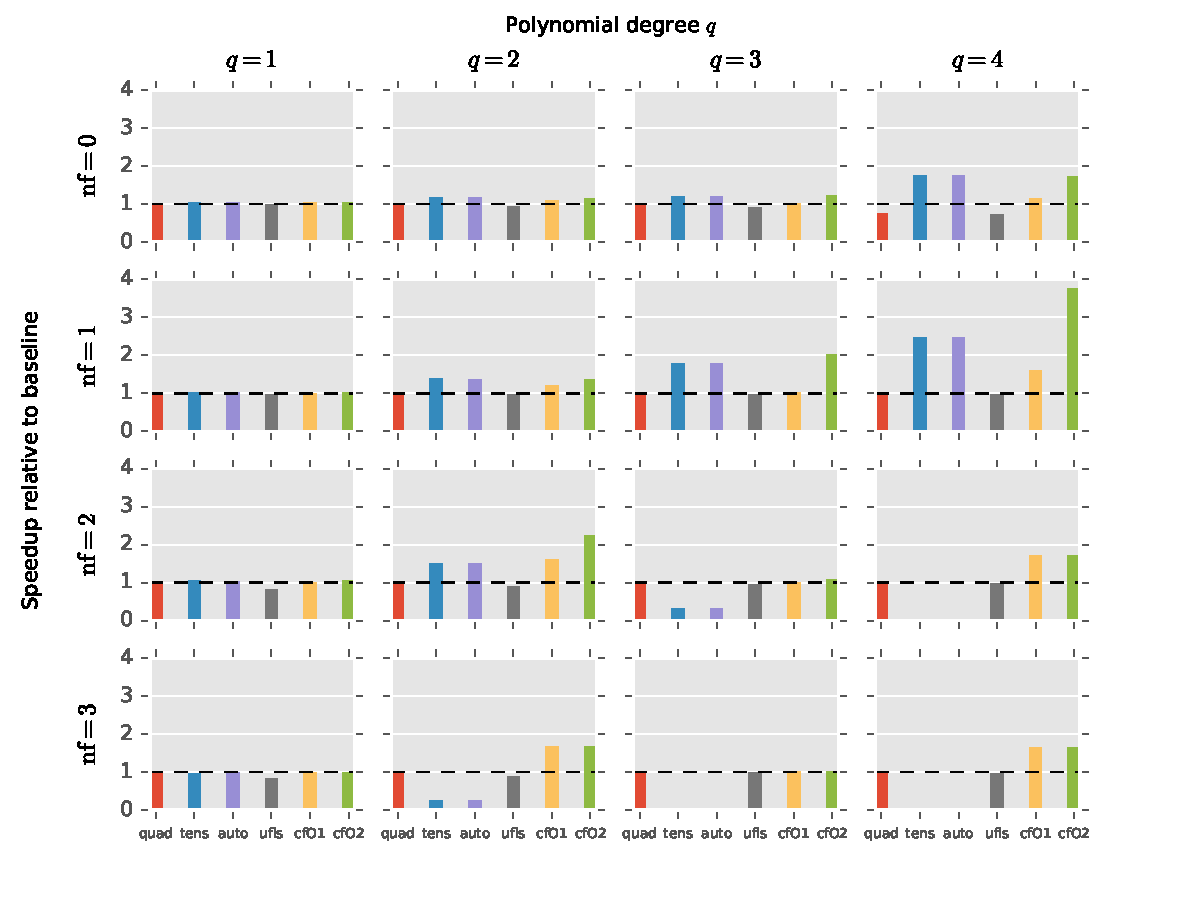
\includegraphics[scale=0.7]{perf-results/mass}
%%\caption{Mass results.}\label{fig:mass}
%\end{figure}
%


\paragraph{Helmholtz}
%\begin{figure}[t]  
%...
%%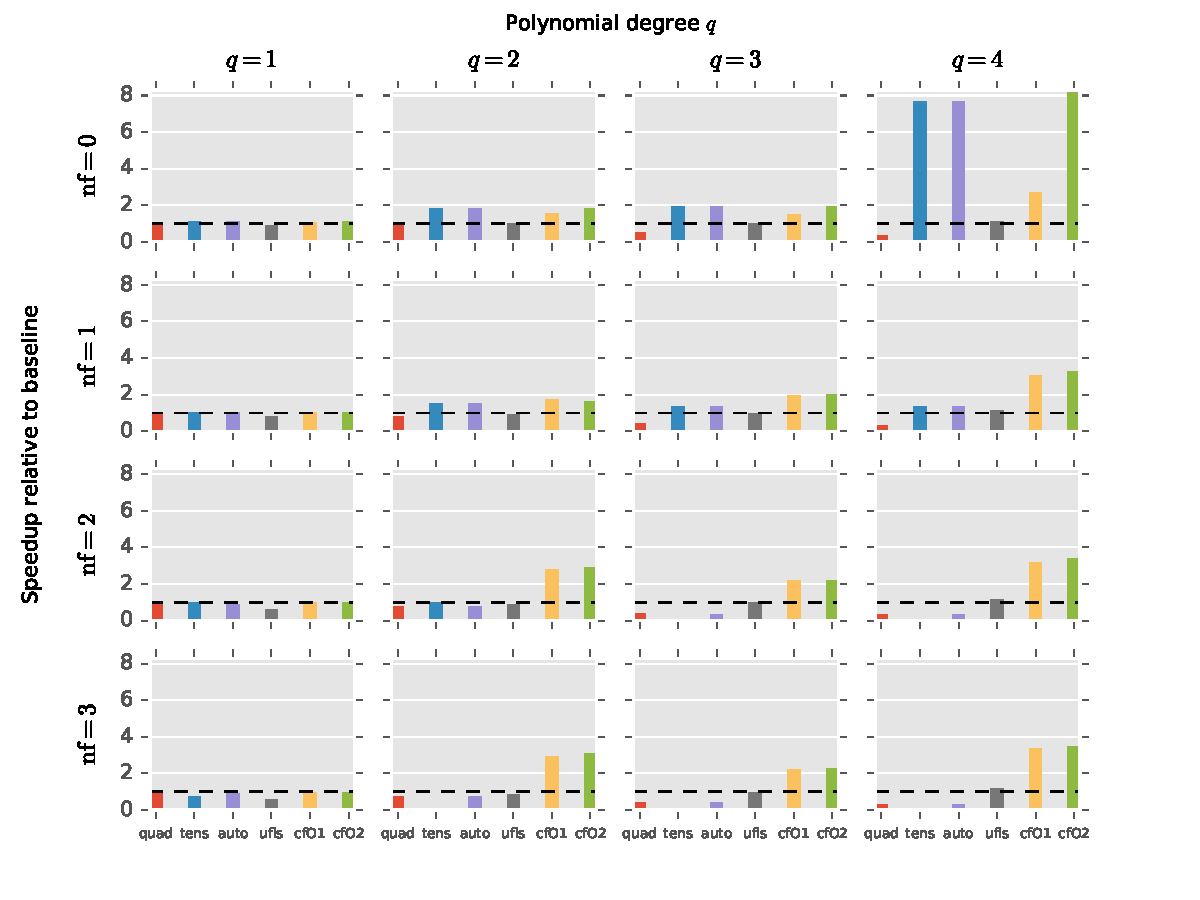
\includegraphics[scale=0.7]{perf-results/helmholtz}
%%\caption{Helmholtz results.}\label{fig:helmholtz}
%\end{figure}
%The results for the Helmholtz problem are provided in Figure~\ref{fig:helmholtz}. We observe that \texttt{ffc} slows the code down, especially for $q \geq 3$. This is a consequence of using indirection arrays in the generated code that, as explained in Section~\ref{sec:zeros}, prevent, among the other compiler optimizations, SIMD auto-vectorization. The \texttt{auto} version results in minimal performance improvements over \texttt{fix} when $nf=0$, unless $q=4$. This is due to the fact that if the loop over quadrature points is relatively small, then close-to-peak performance is obtainable through basic expression rewriting and code specialization; in this circumstance, generalized loop-invariant code motion and padding plus data alignment. The trend changes dramatically as $nf$ and $q$ increase: a more ample spectrum of transformations must be considered to find the optimal local assembly implementation. We will provide details about the selected transformations in the next section.

\paragraph{Elasticity}
%\begin{figure}[t]  
%...
%%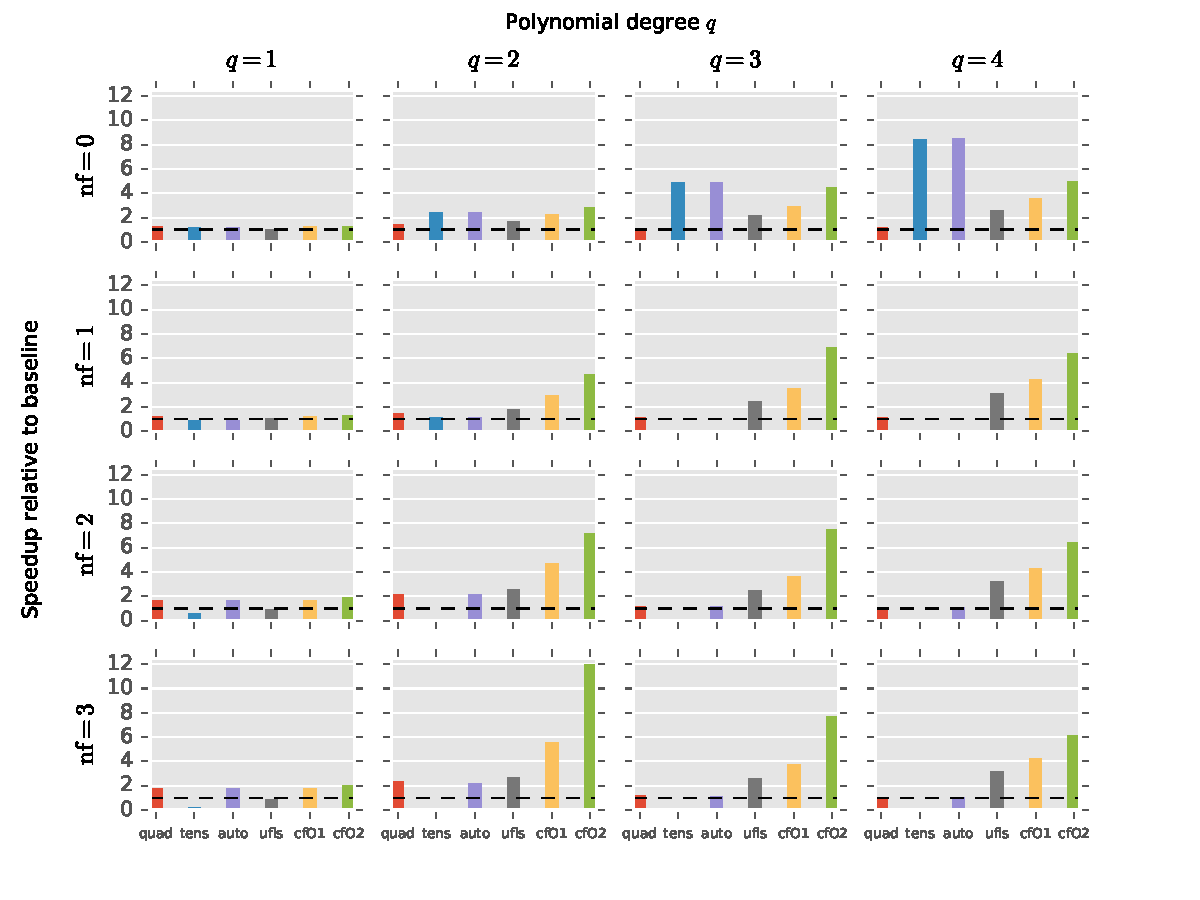
\includegraphics[scale=0.7]{perf-results/elasticity}
%%\caption{Elasticity results.}\label{fig:elasticity}
%\end{figure}
%Figure~\ref{fig:elasticity} illustrates results for the Elasticity problem. This form uses a vector-valued space for the basis functions, so here transformations avoiding computation over zero-valued columns are of key importance. The \texttt{ffc} set of optimizations leads to notable improvements over the original code at $q=1$. The use of inderection arrays allows to phisically eliminate zero-valued columns at code generation time; as a consequence, different tabulated basis functions are merged into a single array. Therefore, despite the execution being purely scalar because of indirection arrays, the reduction in arithmetic intensity and register pressure imply improvement in performance. Nevertheless, \texttt{auto} remains in general the best choice, with gains over \texttt{ffc} that are wider as $p$ and $nf$ increase. 
%
%For $q \geq 2$, in \texttt{ffc} the lack of SIMD vectorization counterbalances the decrease in the number of floating point operations, leading to speed ups over the original code that only occasionally exceed 1$\times$. On the other hand, the successful application of the zero-avoidance optimization while preserving code specialization plays a key role for \texttt{auto}, resulting in much higher performance code especially at $q=2$ and $q=3$. 
%
%It is worth noting that speed ups of \texttt{auto} over \texttt{fix} decrease at $q=4$, particularly for low values of $p$. As we will discuss in Section~\ref{sec:auto-analysis}, this is because at $q=4$ the vector-register tiling transformation (in combination with loop unroll-and-jam) leads to the highest performance. In principle, vector-register tiling can be used in combination to the zero-avoidance technique; however, due to mere technical limitations, this is currently not supported in COFFEE. Once solved, we expect much higher speed ups in the $q=4$ regime as well.





\paragraph{Hyperelasticity}
%\begin{figure}[t]  
%...
%%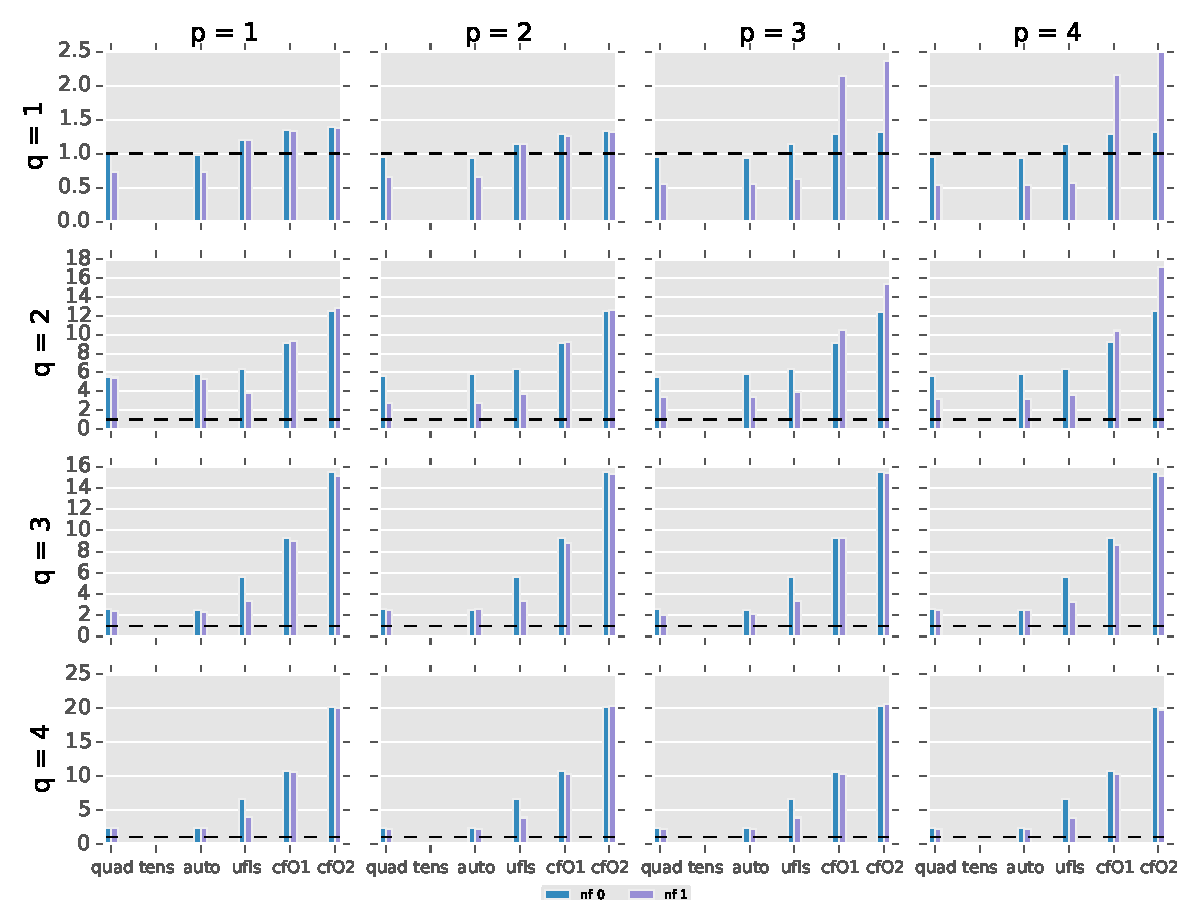
\includegraphics[scale=0.7]{perf-results/hyperelasticity}
%%\caption{Hyperelasticity results.}\label{fig:hyperelasticity}
%\end{figure}
%
%Speed ups for the hyperelasticity form are shown in Figure~\ref{fig:hyperelasticity}. Experiments for $nf \geq 2$ could not be executed because of FEniCS-Form-Compiler's technical limitations. 
%
%For \texttt{auto}, massive speed ups for $q \geq 2$ are to be ascribed to aggressive and successful expression writing. Hyperelasticity problems are really compute-intensive, with thousands of operations being performed, so reductions in redundant and useless computation are crucial. Complex forms like hyperelasticity would benefit from further ``specialized'' optimizations: for example, it is a known technical limitation of COFFEE that, in some circumstances, less temporaries could (should) be generated and that hoisted code could (should) be suitably distributed over different loops to minimize register pressure (e.g. COFFEE could apply loop fission for obtaining significantly better register usage). We expect to obtain considerably faster code once such optimizations will be incorporated. 
%
%In the regime $q \geq 2$ and $nf=1$, peformance improvements are less pronounced moving from $p=1$ to $p=2$, although still significant; in particular, we notice a drop at $p=2$, followed by a raise up to $p=4$. It is worth observing that this effect is common to all sets of optimizations. The hypothesis is that this is due to the way coefficient functions are evaluated at quadrature points (identical in all configurations), which cannot be easily vectorized unless a change in storage layout and loops order is implemented in the code (abstract syntax tree) generator on top of COFFEE. 



\section{Conclusions}
\label{sec:conclusions}
...


% Bibliography
\bibliographystyle{ACM-Reference-Format-Journals}
\bibliography{biblio}


\medskip

\end{document}
